\documentclass{assignment}
\usepackage[pdftex]{graphicx} 
\usepackage{xcolor}
\definecolor{LightGray}{gray}{0.95}
%\usepackage{fancyvrb, minted} 
\usepackage[a4paper, margin = 2.5cm]{geometry} 
\usepackage[T1]{fontenc} 
% set figure path 
\graphicspath{figures}

\usepackage{amsmath, amsfonts, amssymb} 
\usepackage{hyperref, url}  
\usepackage{fancyhdr}
\usepackage{setspace}
\onehalfspacing

\usepackage{subcaption}


\student{Ahmet Akman 2442366}                             
\semester{Spring 2024}                            
\date{\today}                                   

\courselabel{EE449}          
\exercisesheet{Homework 1}{Report}  

\school{Middle East Technical University}        
\university{Electrical and Electronics Engineering}        

%%%%%%%%%%%%%%%%%%%%%%%%%%%%%%%%%%%%%%%%%%-DOCUMENT-%%%%%%%%%%%%%%%%%%%%%%%%%%%%%%%%%%%%%%%%%%%%

\begin{document}


\section{Question 1}

\subsection*{Question 1.1 - Preliminaries}
The partial derivative calculation steps for Tanh, Sigmoid, and ReLU activation functions are shown in Figure \ref{partial_der}.

\begin{figure}[!htb]
    \centering
    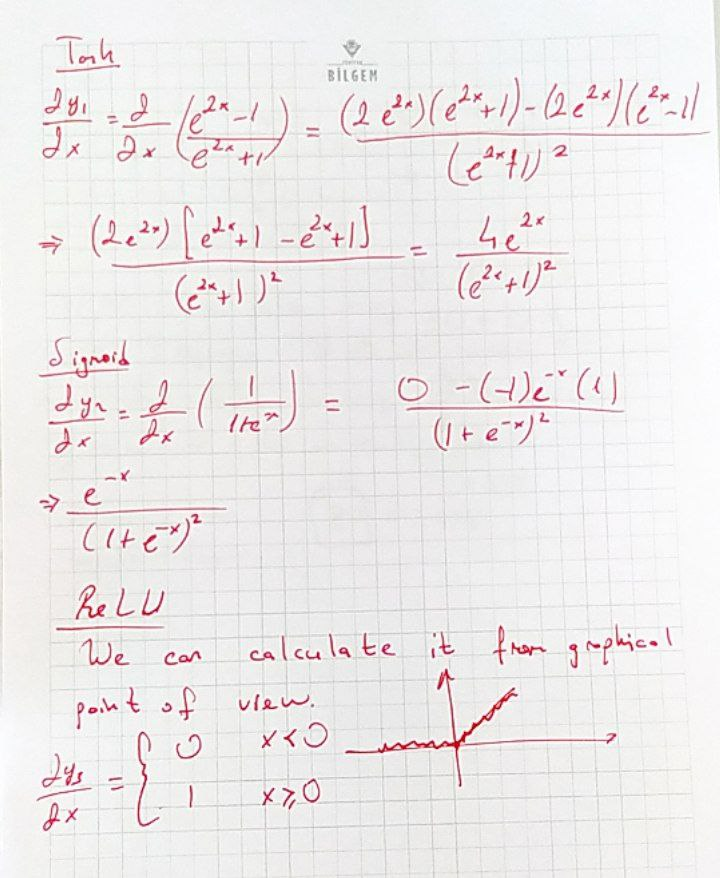
\includegraphics[width=0.6\textwidth]{figures/partial_der.jpg}
    \caption{Partial derivative calculation steps for Tanh, Sigmoid and ReLU activation functions.}
    \label{partial_der}
\end{figure}

Figure \ref{fig:activation_functions} illustrates the activation functions' response between -2 and 2. The plots are obtained using the matplotlib library as instructed.

\begin{figure}[!htb]
    \centering
    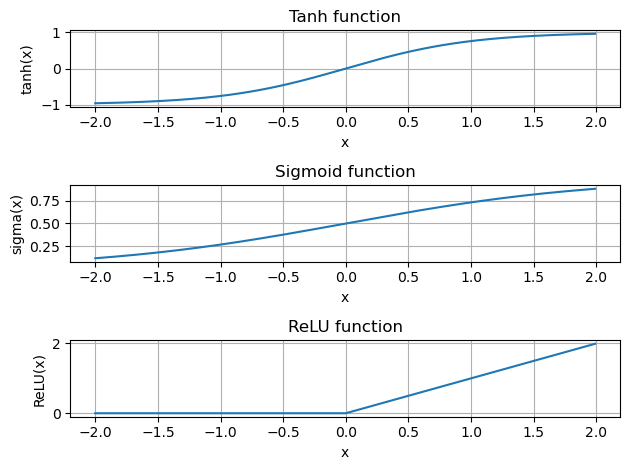
\includegraphics[width=0.75\textwidth]{figures/q1_1.png}
    \caption{Activation functions plot.}
    \label{fig:activation_functions}
\end{figure}

Figure \ref{fig:activation_functions_gradient} indicates the gradients of those functions in the same range. The gradients are calculated using the partial derivatives derived in Figure \ref{partial_der}.

\begin{figure}[!htb]
    \centering
    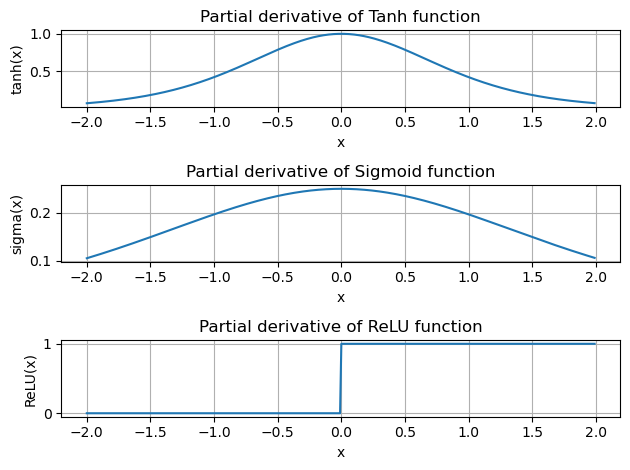
\includegraphics[width=0.75\textwidth]{figures/q1_2.png}
    \caption{Gradients of the activation functions plot.}
    \label{fig:activation_functions_gradient}
\end{figure}



\subsection*{Question 1.2}

In this part, MLP with one hidden layer is implemented utilizing the given code template. The input-output pairs are fetched from the XOR data provided in utils.py. Note that for all networks, the learning rate is fixed at 0.00001, and seed is utilized. Figure \ref{fig:sigmoid_q1} shows the decision boundary for the sigmoid-activated network. 

\begin{figure}[!htb]
    \centering
    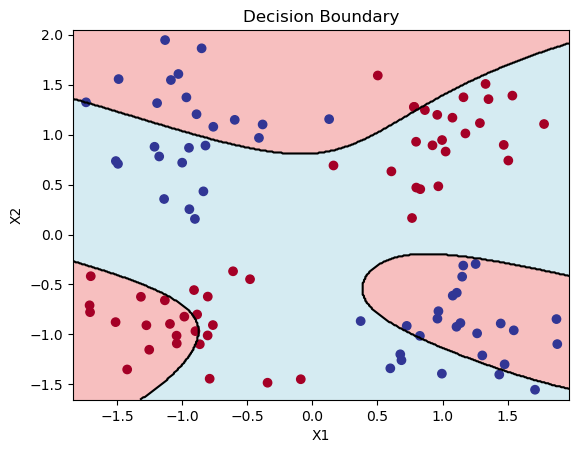
\includegraphics[width=0.8\textwidth]{figures/q1_sigmoid.png}
    \caption{Sigmoid activated XOR problem output.}
    \label{fig:sigmoid_q1}
\end{figure}

Similarly, Figure \ref{fig:tanh_q1} is the decision boundary for the tanh-activated network, and Figure \ref{fig:relu_q1} is the decision boundary for the ReLU-activated network.


\begin{figure}[!htb]
    \centering
    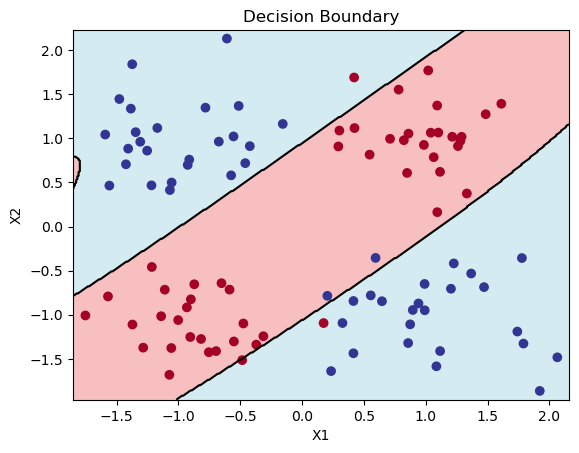
\includegraphics[width=0.8\textwidth]{figures/q1_tanh.png}
    \caption{Tanh activated XOR problem output.}
    \label{fig:tanh_q1}
\end{figure}

\begin{figure}[!htb]
    \centering
    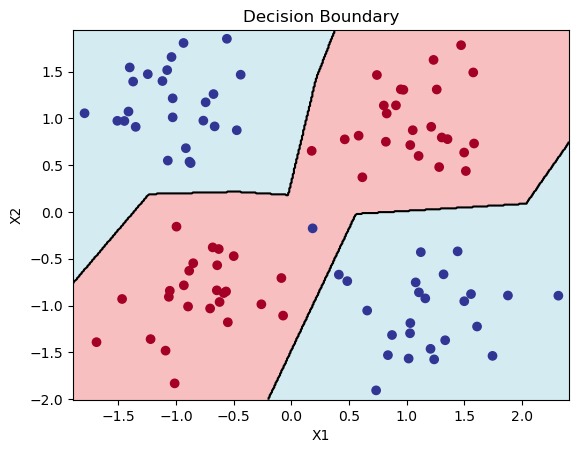
\includegraphics[width=0.8\textwidth]{figures/q1_relu.png}
    \caption{ReLU activated XOR problem output.}
    \label{fig:relu_q1}
\end{figure}

\subsection*{Question 1.3 - Discussions}
\textbf{1.}
All of those activation functions provide a smooth transition from one state to another. The advantage of Tanh and Sigmoid is they are limited in the range of -1 to 1 and 0 to 1, respectively. This property can be beneficial in some cases. However, the ReLU function is not limited in the range. It is also computationally cheaper than the other two. The disadvantage of ReLU is that it is not smooth at the origin. This can cause some problems in the optimization process. Another advantage of ReLU is negative gradients are zero. This may be helpful in some cases. 


\textbf{2.}
\noindent XOR problem is an input decision problem where inputs have to be different than each other to obtain 1. Since the output is always with respect to the state of two variables, the decision boundary is not linear. Therefore, a single-layer perceptron can not be solved since, in one step, two case evaluations can not be done. Yet, by adding a hidden layer, the problem is solved. The activation functions are used to introduce non-linearity to the network. The decision boundary of the XOR problem is shown in Figures \ref{fig:sigmoid_q1}, \ref{fig:tanh_q1} and \ref{fig:relu_q1}. As can be seen from the figures, the MLPs with activation functions can solve the XOR problem to some extent.

\textbf{3.}
\noindent The boundaries change in each run since the initial weights and the data points are randomly generated. Therefore, the decision boundaries are dependent on the training process, where initial randomness leads to different outputs.


\section{Question 2}
A convolution operator is implemented using a set of nested loops. The outputs are checked on a separate code so that they are identical to the output of torch.conv2d. Using the provided inputs, outputs provided in Figure \ref{fig:convolution_out} are obtained.

% 10 subfigure figure

\begin{figure}[!htb]
    \begin{subfigure}{0.3\textwidth}
        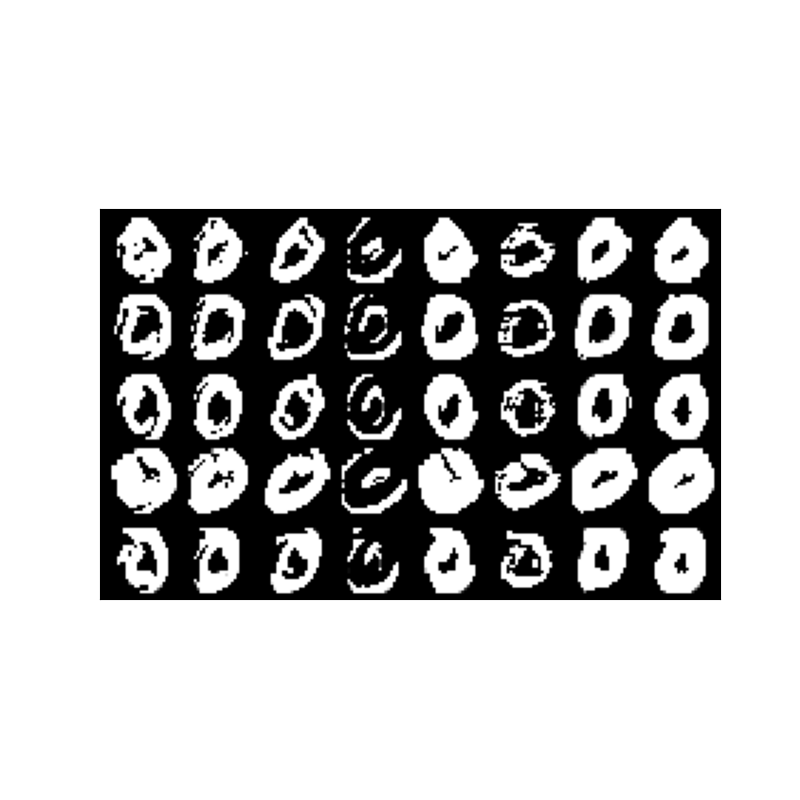
\includegraphics[width=\textwidth]{figures/out_0.png}
        \caption{Output 0}
    \end{subfigure}\hfill
    \begin{subfigure}{0.3\textwidth}
        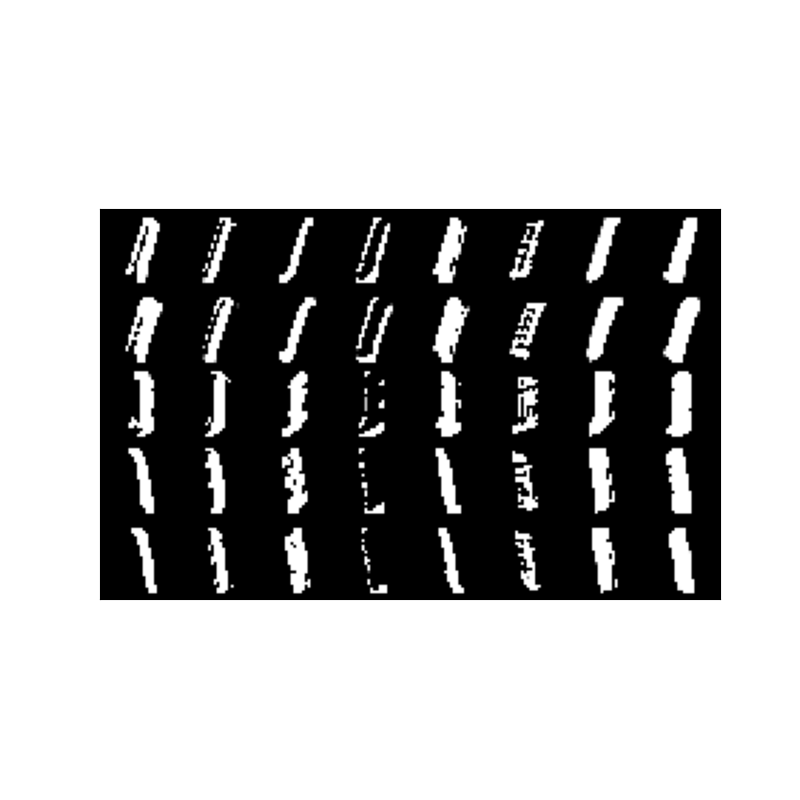
\includegraphics[width=\textwidth]{figures/out_1.png}
        \caption{Output 1}
    \end{subfigure}\hfill
    \begin{subfigure}{0.3\textwidth}
        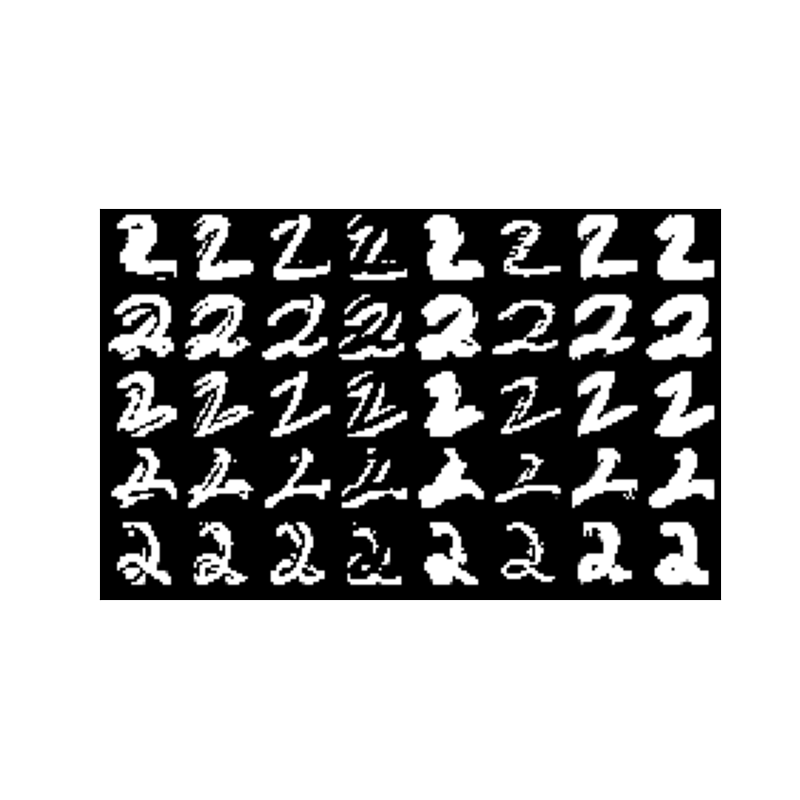
\includegraphics[width=\textwidth]{figures/out_2.png}
        \caption{Output 2}
    \end{subfigure}
    \vskip\baselineskip
    \begin{subfigure}{0.3\textwidth}
        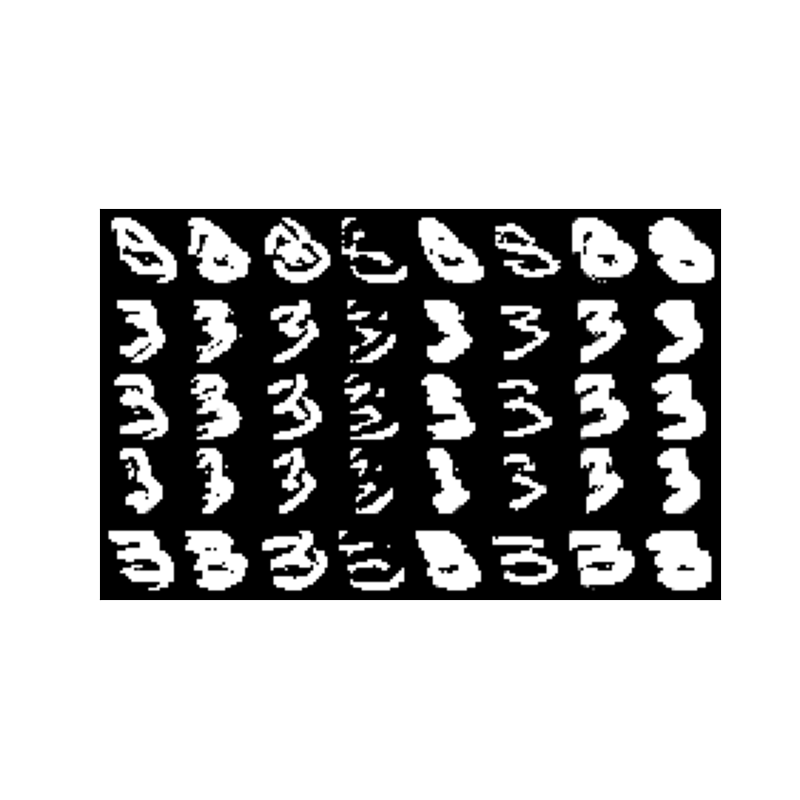
\includegraphics[width=\textwidth]{figures/out_3.png}
        \caption{Output 3}
    \end{subfigure}\hfill
    \begin{subfigure}{0.3\textwidth}
        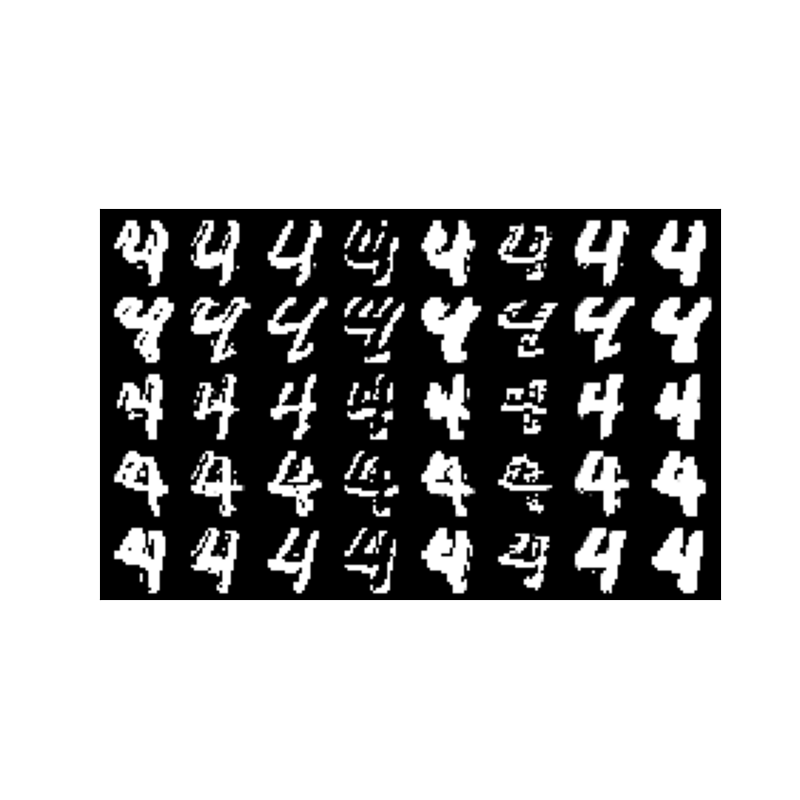
\includegraphics[width=\textwidth]{figures/out_4.png}
        \caption{Output 4}
    \end{subfigure}\hfill
    \begin{subfigure}{0.3\textwidth}
        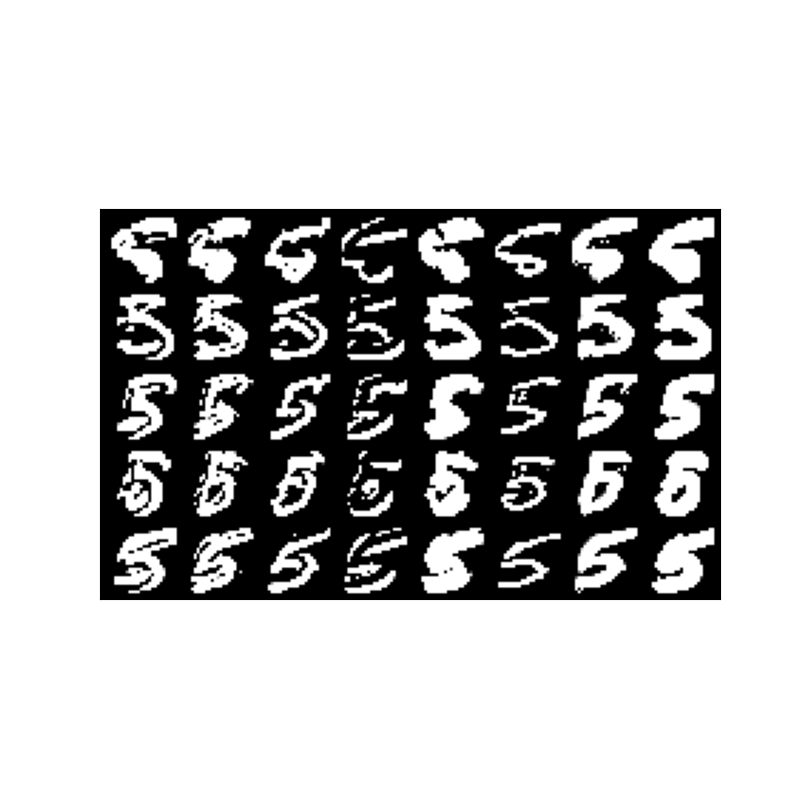
\includegraphics[width=\textwidth]{figures/out_5.png}
        \caption{Output 5}
    \end{subfigure}
    \vskip\baselineskip
    \begin{subfigure}{0.3\textwidth}
        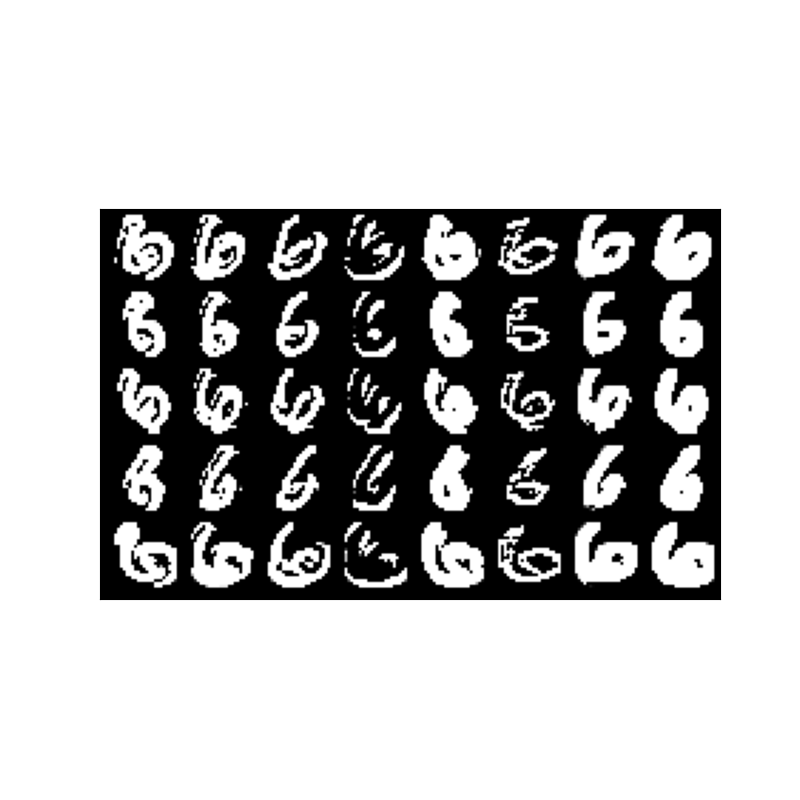
\includegraphics[width=\textwidth]{figures/out_6.png}
        \caption{Output 6}
    \end{subfigure}
    \hfill
    \begin{subfigure}{0.3\textwidth}
        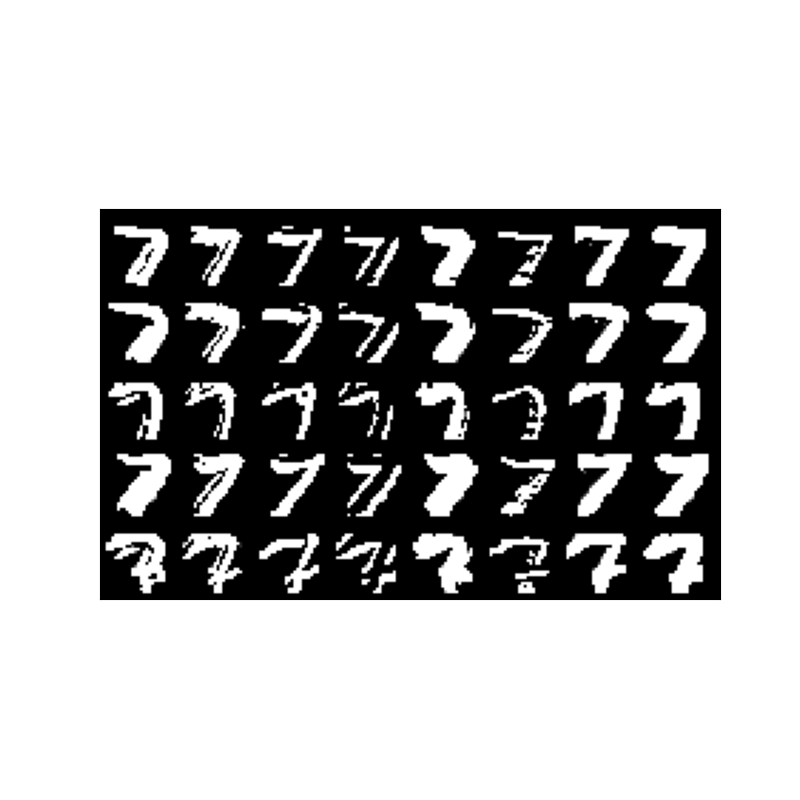
\includegraphics[width=\textwidth]{figures/out_7.png}
        \caption{Output 7}
    \end{subfigure}\hfill
    \begin{subfigure}{0.3\textwidth}
        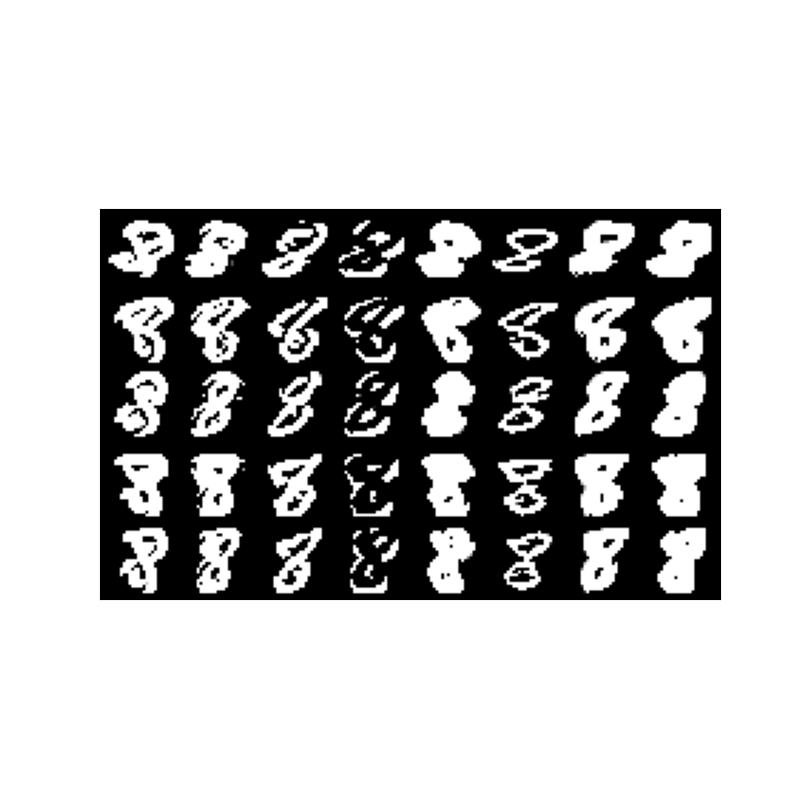
\includegraphics[width=\textwidth]{figures/out_8.png}
        \caption{Output 8}
    \end{subfigure}
    % \vskip\baselineskip
    % \begin{subfigure}{0.3\textwidth}
    %     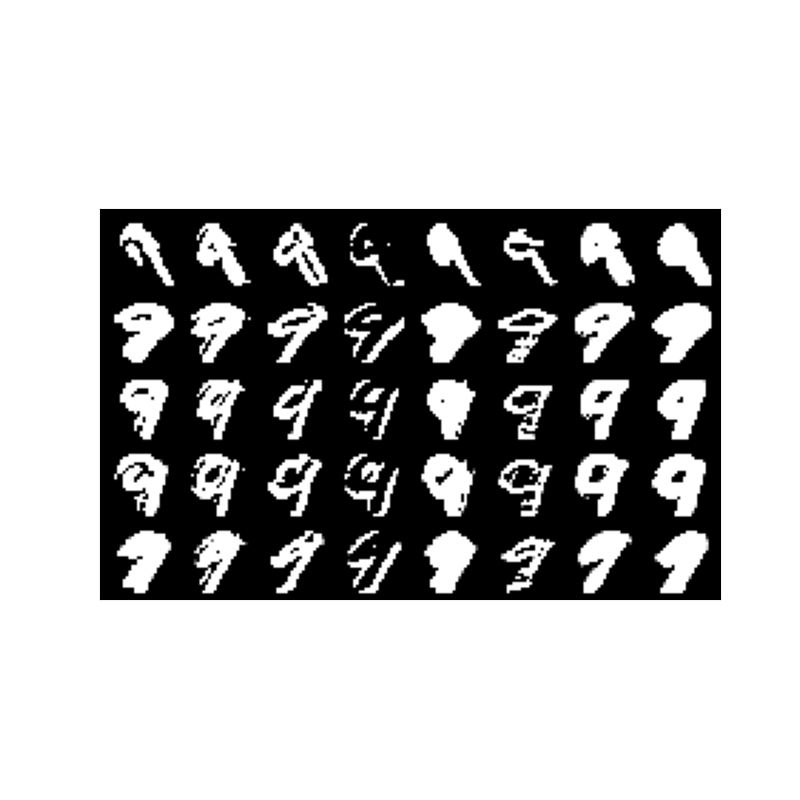
\includegraphics[width=\textwidth]{figures/out_9.png}
        
    %     \caption{Output 9}
    % \end{subfigure}\hfill
    \caption{Convolution output}
    \label{fig:convolution_out}
\end{figure}

\subsection*{Question 2.2 - Discussions}
\textbf{1.}
Two-dimensional convolution operation provides filtering in two dimensions via a kernel. The kernel is applied to the input image in a sliding window fashion. The output is obtained by element-wise multiplication of the kernel and the input image. The kernel is then shifted by a stride, and the process is repeated. That is, two-dimensional convolution operations with learnable kernel entries are commonly used in image processing to extract features from the image. The kernel is learned during the training process. Those feature maps encode necessary information about distinct clues in the image. For example, in the case of object recognition, a specific kernel can be trained to detect bicycle rims. 
The kernel of a convolution layer corresponds to the filter function in one dimension. It is used to suppress or enhance certain information in the input image.

\textbf{2.}
\noindent The sizes of the kernel correspond to the size of the filter. Therefore, the size list can be explained as follows (batch size, input channels, output channels, filter height, filter width). Batch size is the number of input sets in a batch if batching is used; we have not utilized it here. Input channels are the number of depth dimensions in the image; for example, in RGB frames, it is three. This might be different for different sensor inputs and representations. The output channel number determines the depth dimension of the output tensor. The filter height and width are the dimensions of the filter.

\textbf{3.}
To understand what exactly happened here, let us plot the kernel and input for the number zero. Figure \ref{fig:kernel_input} illustrates the plot.

\begin{figure}[!htb]
    \begin{subfigure}{0.5\textwidth}
        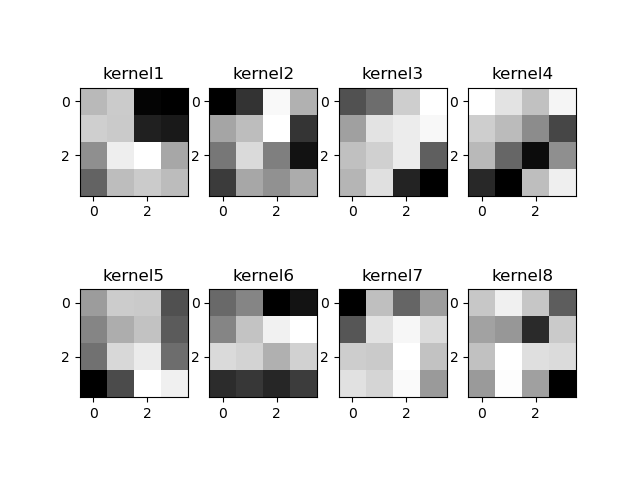
\includegraphics[width=\textwidth]{figures/q2_kernels.png}
        \caption{Kernels}
    \end{subfigure}\hfill
    \begin{subfigure}{0.5\textwidth}
        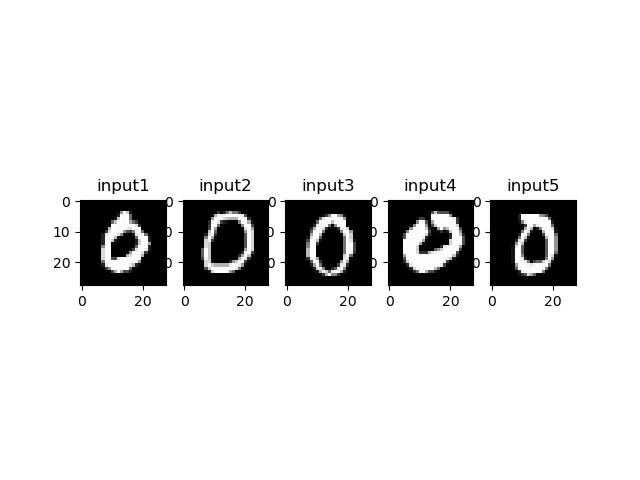
\includegraphics[width=\textwidth]{figures/q2_zero_input.png}
        \caption{Input set for number zero.}
    \end{subfigure}
    \caption{Kernel and input for number zero.}
    \label{fig:kernel_input}
\end{figure}

\noindent When we have a look at what the output image represents, on each row, an input image is convolved with a kernel. Different kernels are applied to the input image. The output image is the result of those convolutions. Figure \ref{fig:kernel_input} shows the input and kernel pairs in order.

\textbf{4.}
\noindent Each convolution kernel embeds a certain feature of the image. That is, if we have a look at Figure \ref{fig:kernel_input}.a, we can see that kernel 4 enhances the contours on the image, whereas kernel 6 enhances the filled part of those contours. This is the reason why we see similarly formatted outputs in the same column.

\textbf{5.}
\noindent Similarly, since we "highlight" different properties on the image without filters, we see different patterns on the output side, even if the input is the same.

\textbf{6.}
So, we can interpret from 4 and 5 that the output of the convolution layer is the result of the feature extraction process. The output is the result of the convolution of the input image with the learned filters. The output is the feature map that encodes the information about the input image. By post-processing those feature maps, we can obtain the necessary interpretations of the input image.

\section{Question 3}
\subsection*{Question 3.1}
The implementations related to each architecture are completed as instructed. The code is given in the appendix. As a result, the plot shown in Figure \ref{Q3} is obtained. Also, the first layer weights recorded are plotted and shown in Figure \ref{fig:weights}.

\begin{figure}[!htb]
    \centering
    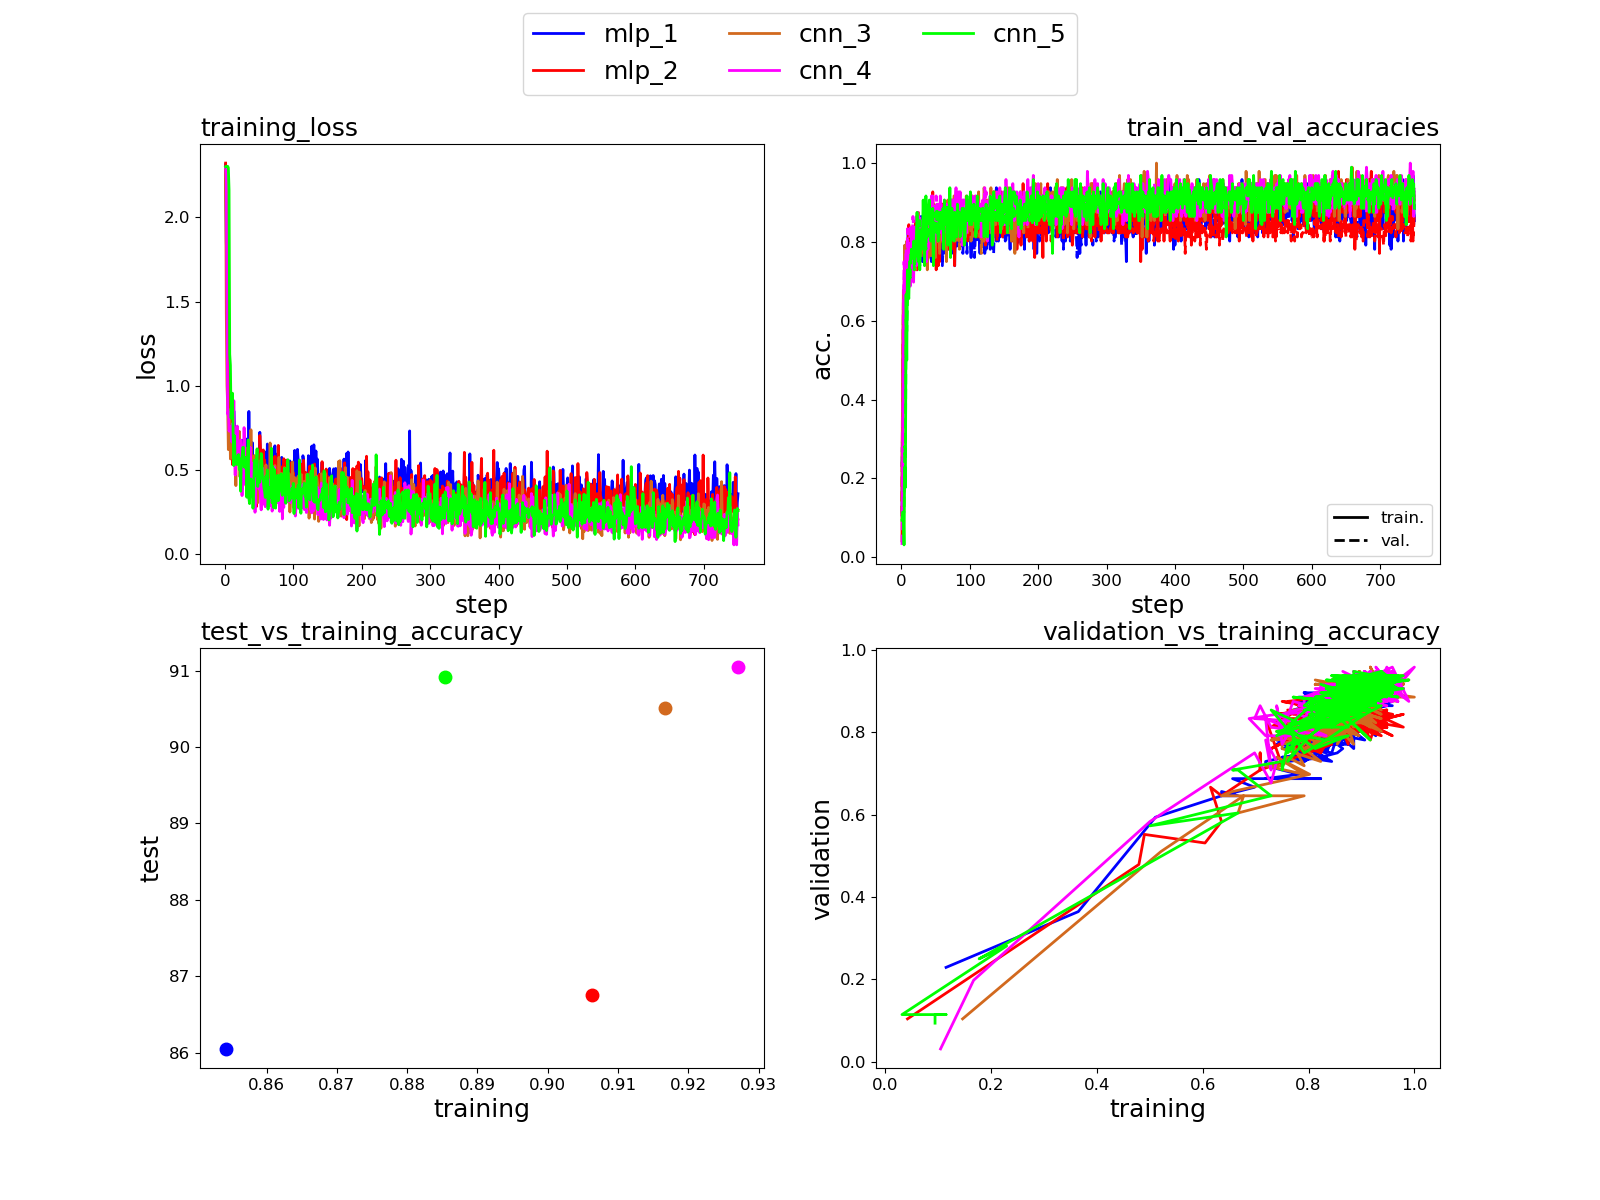
\includegraphics[width=1\textwidth]{figures/q3_results.png}
    \caption{Benchmark of five different architectures.}
    \label{Q3}
\end{figure}


\begin{figure}[!htb]
    \begin{subfigure}{0.5\textwidth}
        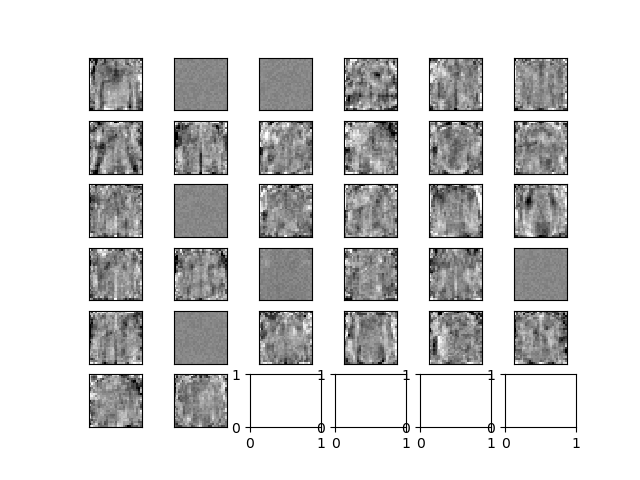
\includegraphics[width=\textwidth]{figures/weights_mlp_1.png}
        \caption{mlp 1}
    \end{subfigure}\hfill
    \begin{subfigure}{0.5\textwidth}
        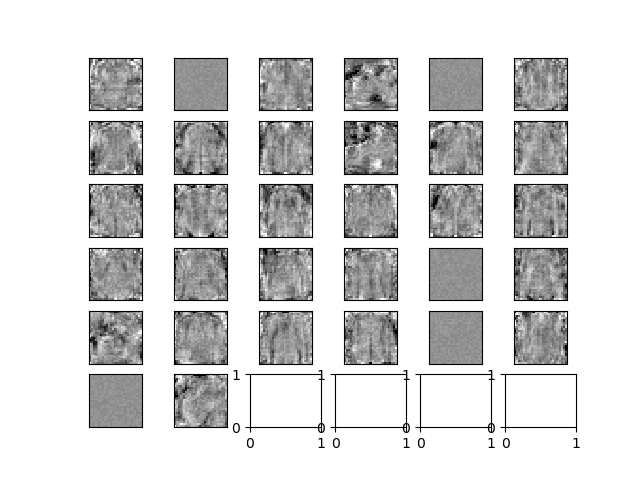
\includegraphics[width=\textwidth]{figures/weights_mlp_2.png}
        \caption{mlp 2}
    \end{subfigure}\vskip\baselineskip
    \begin{subfigure}{0.3\textwidth}
        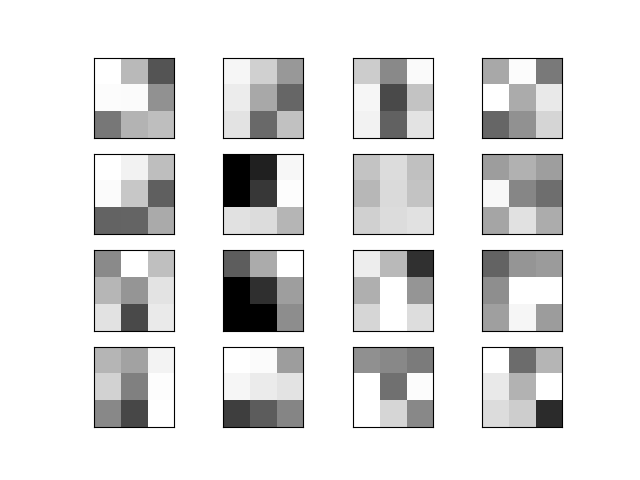
\includegraphics[width=\textwidth]{figures/weights_cnn_3.png}
        \caption{cnn 3}
    \end{subfigure}
    \hfill
    \begin{subfigure}{0.3\textwidth}
        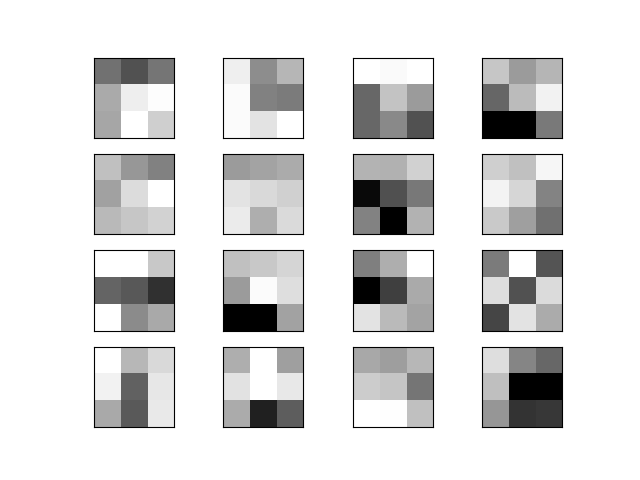
\includegraphics[width=\textwidth]{figures/weights_cnn_4.png}
        \caption{cnn 4}
    \end{subfigure}\hfill
    \begin{subfigure}{0.3\textwidth}
        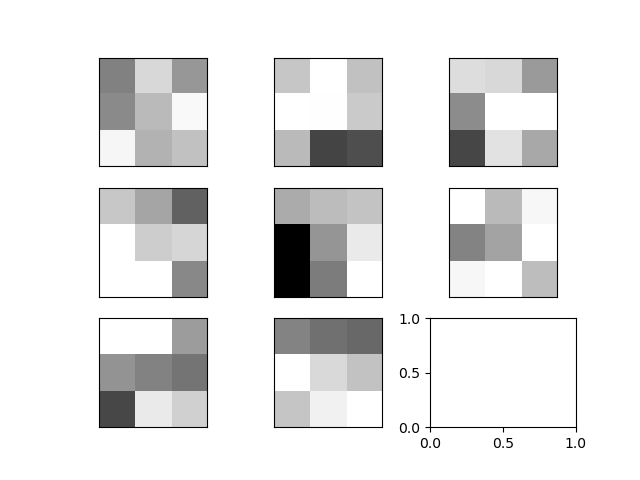
\includegraphics[width=\textwidth]{figures/weights_cnn_5.png}
        \caption{cnn 5}
    \end{subfigure}\hfill
    \caption{Weights of the first layers.}
    \label{fig:weights}
\end{figure}

\subsection*{Question 3.2 - Discussions}

\textbf{1.}
The generalization performance of a classifier is the ability of the classifier to perform well on unseen data. That is, the classifier should be able to generalize the patterns in the training data to the test data. The overfitting phenomenon is the case where the model fits the training data too much and loses its generalization.

\textbf{2.}
\noindent The plots, test vs. training accuracy and validation vs. training accuracy are the most informative in this sense.


\textbf{3.}
\noindent Somehow, the validation vs training accuracy plot is hard to read out. Therefore, deductions are made from test vs training accuracy plots. First of all, one can see right away that the plot that CNN-based models generalized better, whereas MLP-based ones have testing accuracy lower than training accuracy. On the other hand, amongst CNN-based ones, cnn4 has the best accuracy in terms of both training and test accuracy. However, it can be deduced that cnn5 has the best generalization performance since it has quite high test accuracy compared to its training accuracy. The test scores are even better than the training scores. 


\textbf{4.}

\begin{table}[h]
    \centering
    \begin{tabular}{|c|c|}
    \hline
    \textbf{Architecture} & \textbf{Trainable Params} \\
    \hline
    mlp 1 & 25,450 \\
    mlp 2 & 27,818 \\
    cnn 3 & 22,626 \\
    cnn 4 & 14,962 \\
    cnn 5 & 10,986 \\
    \hline
    \end{tabular}
    \caption{Trainable Parameters of Different Architectures}
    \label{table:TrinableParams}
\end{table}


\noindent As the number of parameters increases, the number of points to fit the data increases. Therefore, the model can fit the data better in the most basic setting. The number of parameters for each architecture is given in Figure \ref{table: TrinableParams}. So, classification performance increases as the number of parameters increases to a certain point, as we can observe from multi-layer perceptron training. From cnn3 to cnn4, both training and test accuracy increases, but a number of parameters are lower in cnn4. However, from cnn4 to cnn5, the test accuracy is almost the same, whereas the training accuracy decreases considerably. Therefore, it can be said that using only a number of parameters to describe generalization and training capabilities is not the best idea. 

\textbf{5.}
\noindent As the depth of the network increases, e.g., from mlp1 cnn5 network depth increases, in general, both classification performance increases up to a certain level and then decreases. For generalization, we can say that it always increases according to the data we have right now in those examples. 


\textbf{6.}
\noindent The mlp weights are not interpretable. However, one may interpret what kind of filtering is done by the CNN weights by looking at the plots shown in Figure \ref{fig:weights}. The first layers, in general, encode the most basic features like cırbers, edges, and so on.

\textbf{7.}
\noindent The limited experience of the report writer does not allow them to extract the information on whether the filters are specific to the cases by looking at them. However, principally, certain CNN filters are trained to detect certain features in the input image. Again, the first layers encode the most simplistic features like cırbers and edges. Therefore, the filters are specific to the classes to distinguish them better. 

\textbf{8.}
\noindent Similarly, it is hard to distinguish between the filters by looking at the weights. The most interpretable ones are from the cnn4 architecture. The filters are more clear in this case.

\textbf{9.}
\noindent The mlp1 and mlp2 are the simplest architectures that are similar to each other. The mlp2 introduces one more layer. The cnn3, cnn4, and cnn5 are the convolutional neural network architectures. The cnn3 has three layers with three different spatial kernels. The cnn5 has six convolutional layers with fixed spatial dimensions, but it is the deepest of all five of the architectures. As done in the previous sections, mlp2 performs better than mlp1 by increasing the number of parameters. Cnn4 performs better than cnn3 while having similar number parameters and having higher depth. Cnn5 has a significantly low number of parameters, so it underfits the training set but generalizes quite nicely.

\textbf{10.}
\noindent I would pick cnn4 since it has the best test accuracy and generalization performance. It seems it can fit the data well and does not overfit in this setting.

\section{Question 4}

\subsection*{Question 4.1}
As instructed in the homework documentation, the implementation for both ReLU and sigmoid activate models is done. Necessary statistics are recorded. As a result, the plot shown in Figure \ref{fig:q4} is obtained. Note that the utils.py had to be modified (alpha value edited) to have a proper distinction. Also, Figure \ref{fig:q4_ind} illustrates the individual results for each architecture.

\begin{figure}[!htb]
    \centering
    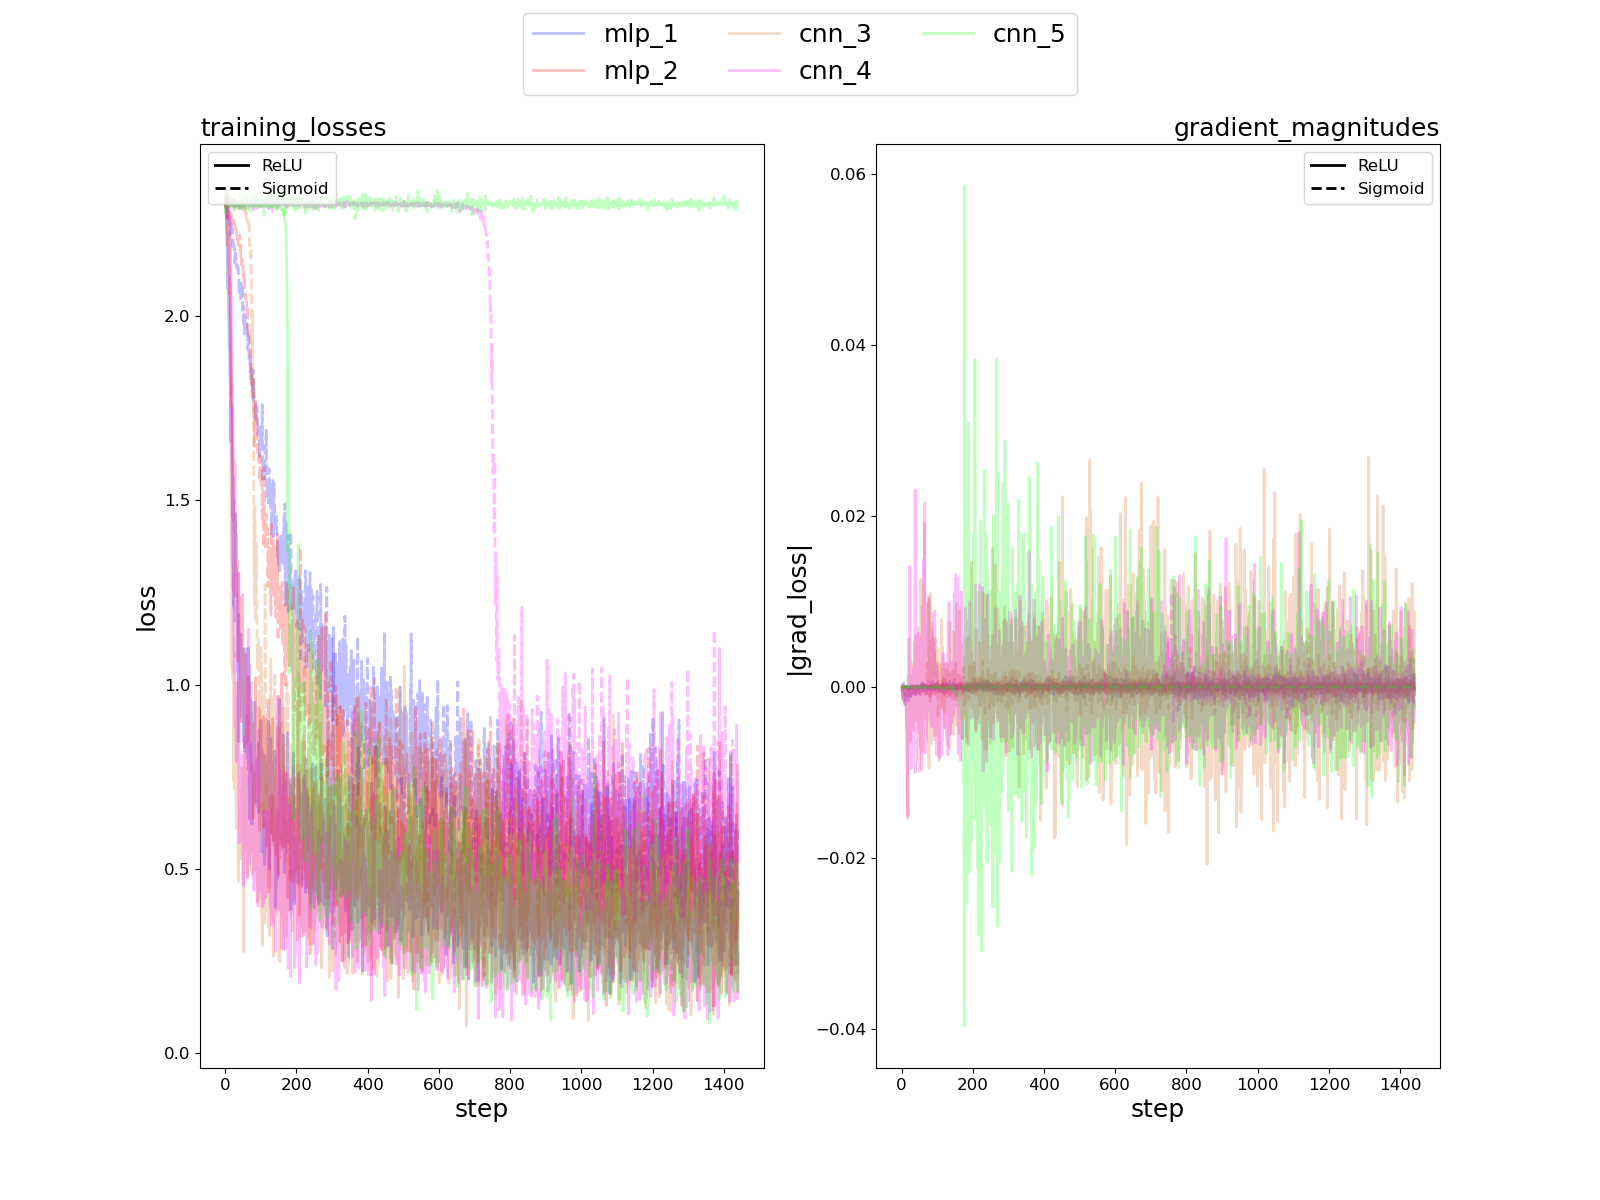
\includegraphics[width=1\textwidth]{figures/part4_alpha.png}
    \caption{Benchmark of five different architectures trained using ReLU and Sigmoid activation functions.}
    \label{fig:q4}
\end{figure}



\begin{figure}[!htb]
    \begin{subfigure}{0.5\textwidth}
        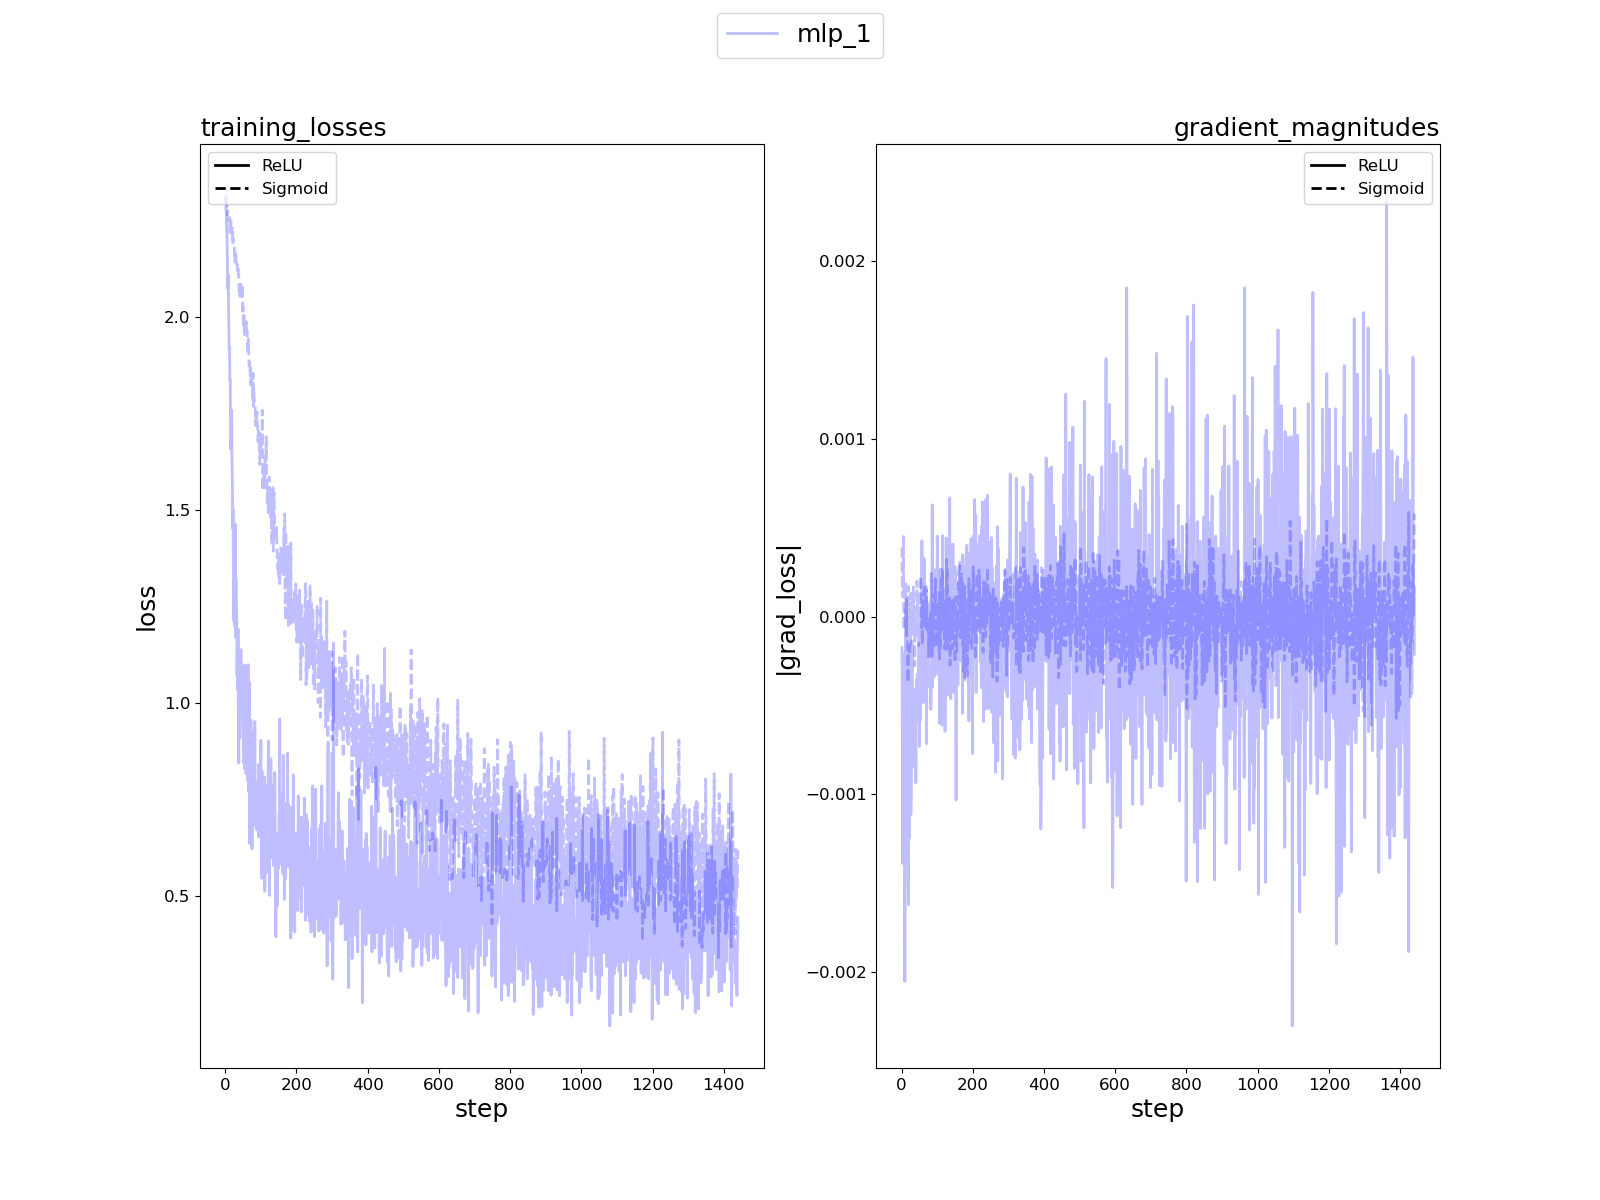
\includegraphics[width=\textwidth]{figures/part4_alpha_mlp_1.png}
        \caption{mlp 1}
    \end{subfigure}\hfill
    \begin{subfigure}{0.5\textwidth}
        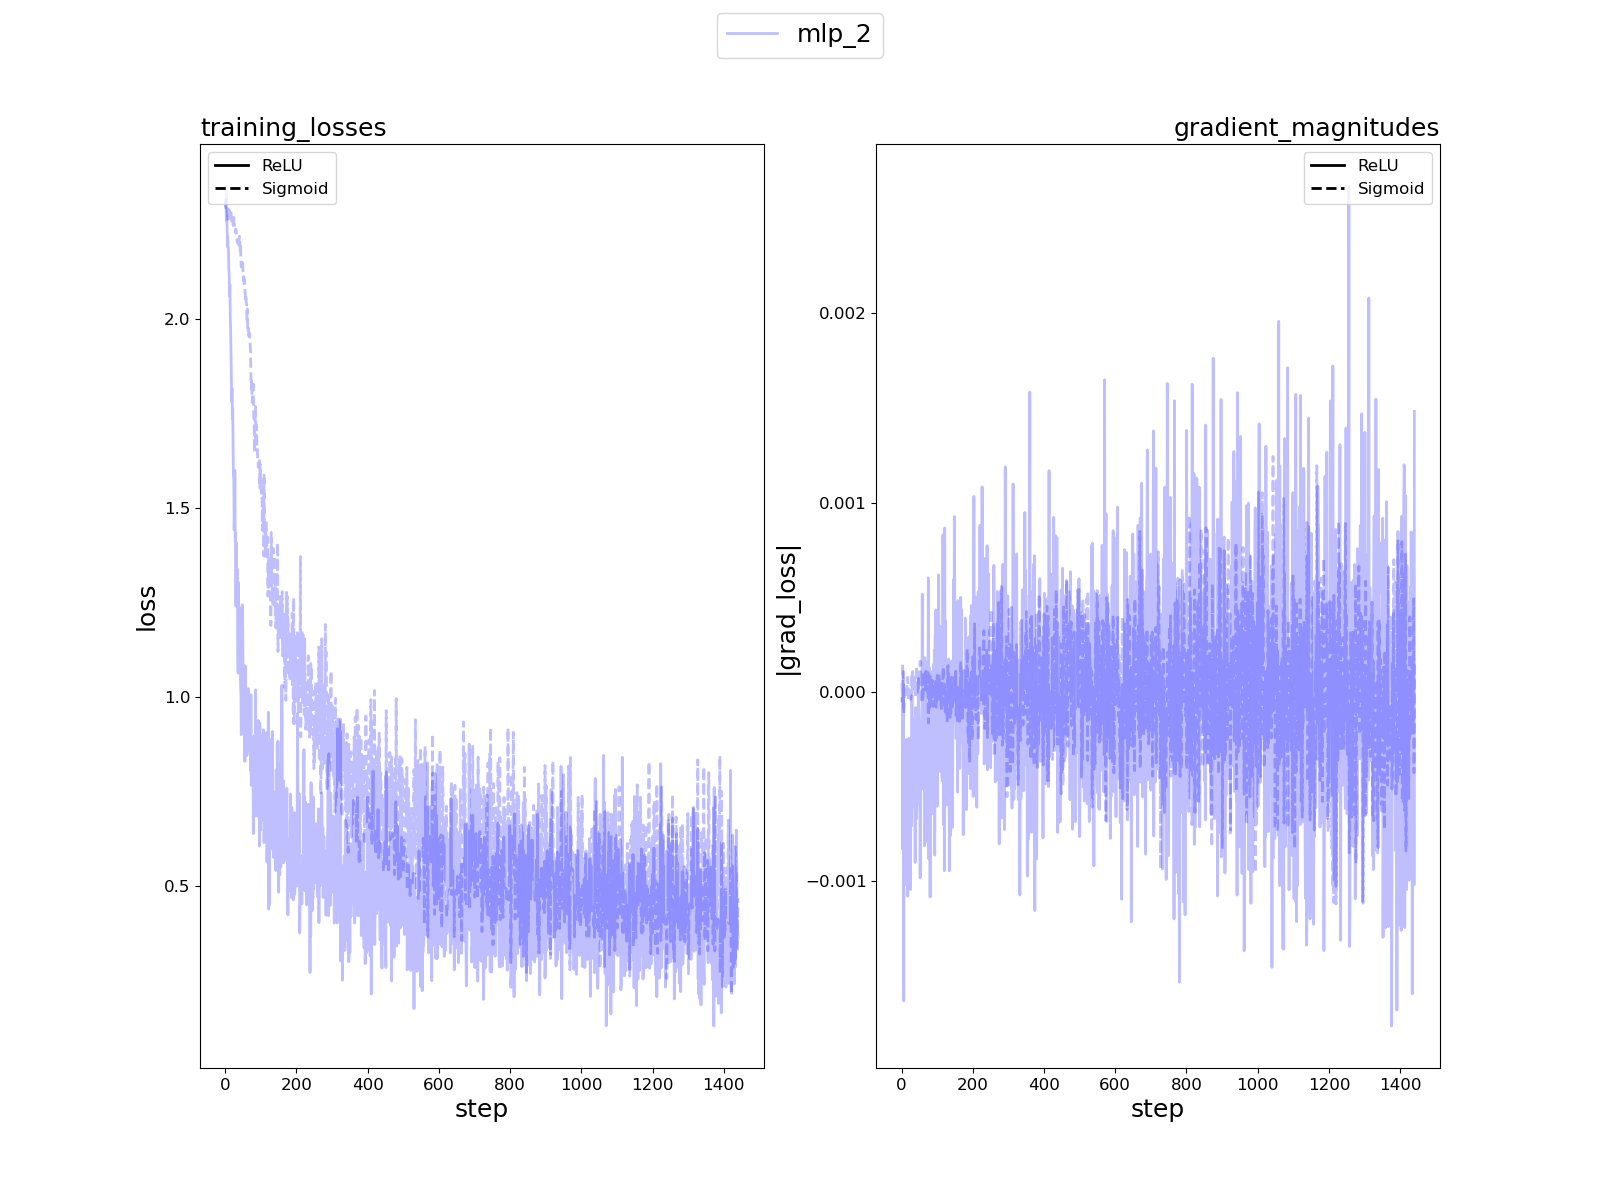
\includegraphics[width=\textwidth]{figures/part4_alpha_mlp_2.png}
        \caption{mlp 2}
    \end{subfigure}\vskip\baselineskip
    \begin{subfigure}{0.3\textwidth}
        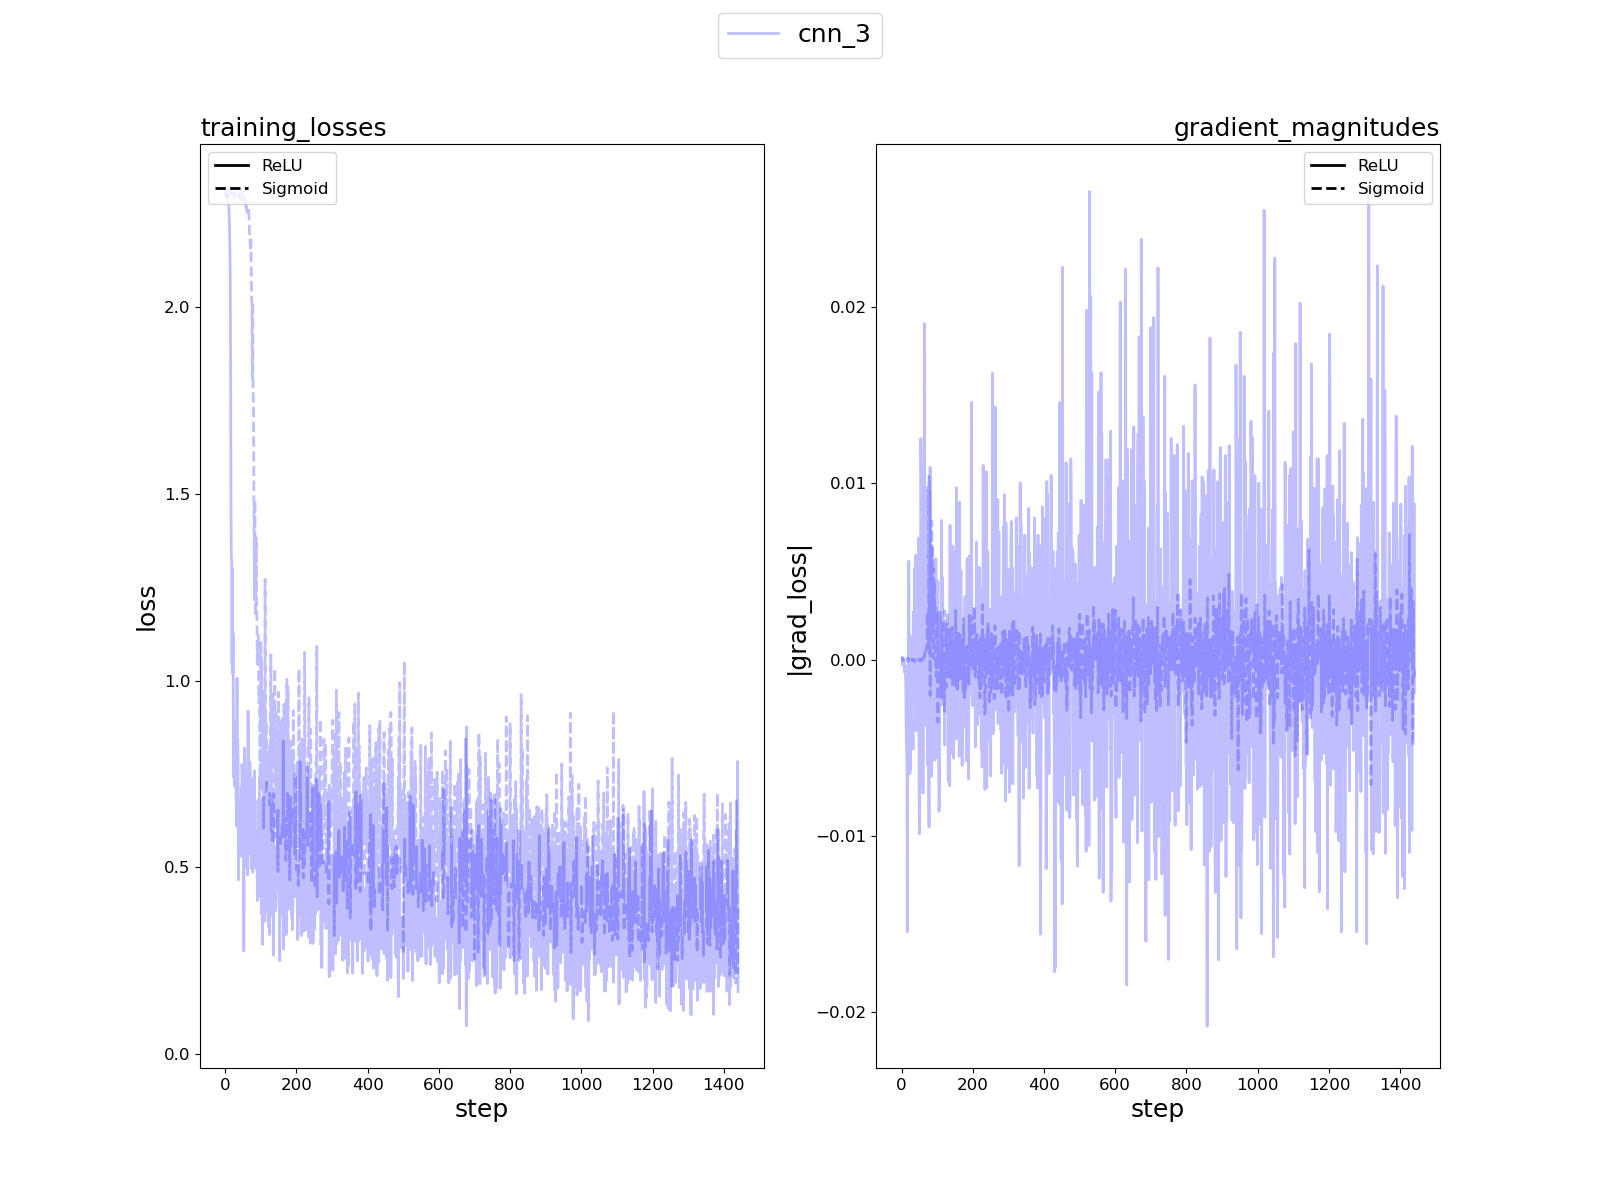
\includegraphics[width=\textwidth]{figures/part4_alpha_cnn_3.png}
        \caption{cnn 3}
    \end{subfigure}
    \hfill
    \begin{subfigure}{0.3\textwidth}
        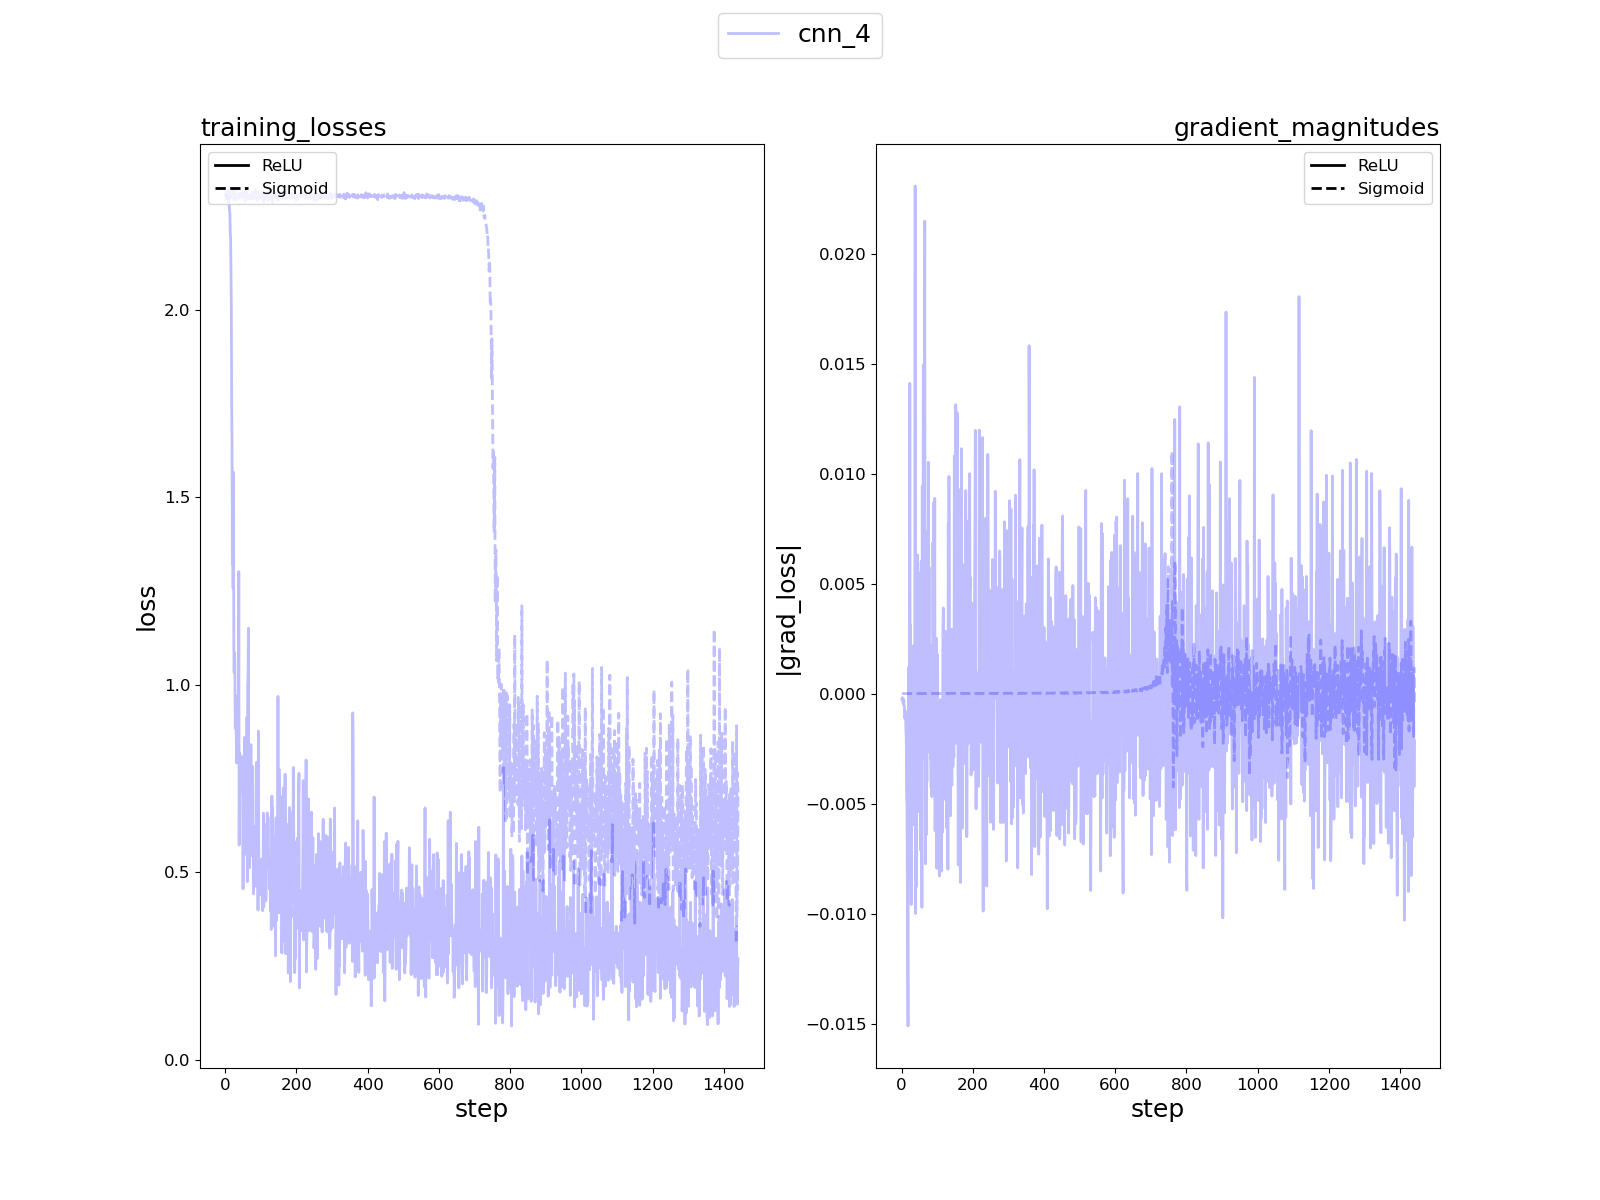
\includegraphics[width=\textwidth]{figures/part4_alpha_cnn_4.png}
        \caption{cnn 4}
    \end{subfigure}\hfill
    \begin{subfigure}{0.3\textwidth}
        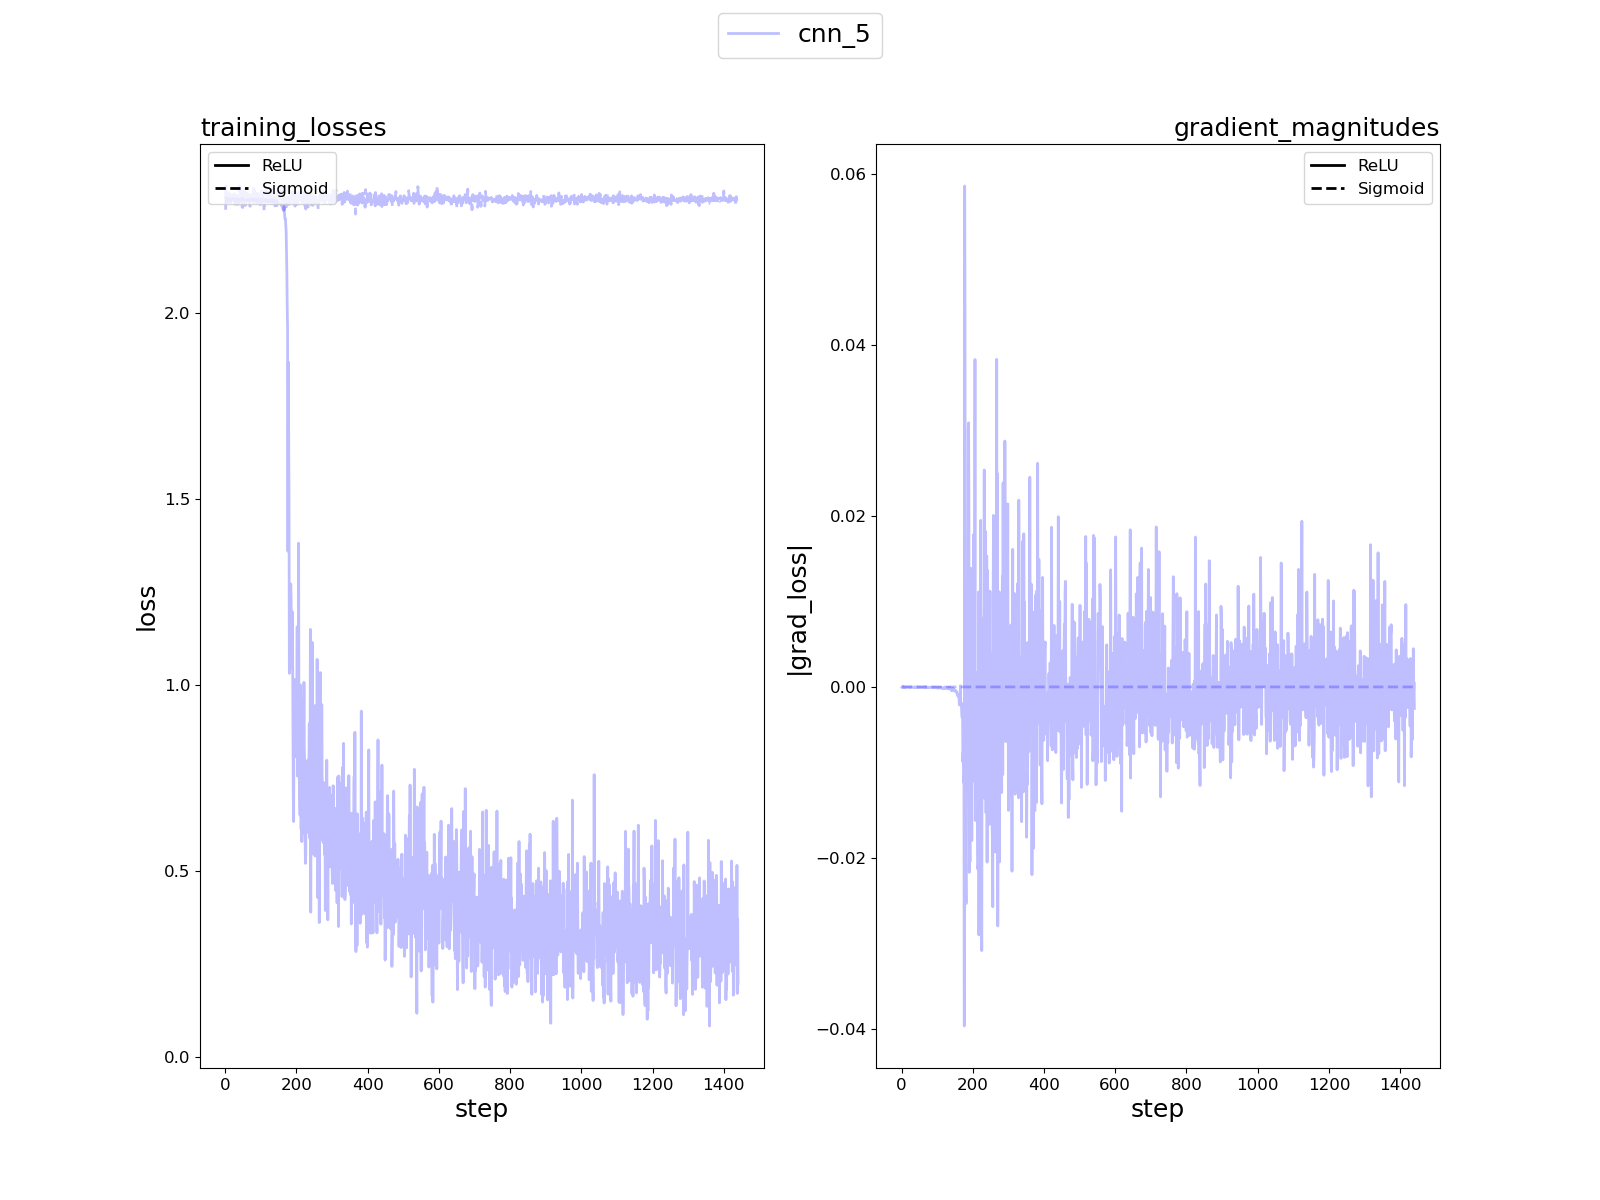
\includegraphics[width=\textwidth]{figures/part4_alpha_cnn_5.png}
        \caption{cnn 5}
    \end{subfigure}\hfill
    \caption{ReLU vs Sigmoid for each architecture.}
    \label{fig:q4_ind}
\end{figure}

\subsection*{Question 4.2 - Discussions}

\textbf{1. -- 2.}
\noindent Gradient behavior is similar in each architecture if we focus on ReLU-activated ones. The values fluctuate around the 0 line as expected. However, the sigmoid-activated ones exhibit different behaviors. The gradients are quite small. Also, as the depth increases, the gradients for sigmoid-activated ones get smaller and quite close to 0. This is due to the vanishing gradient problem. The gradients are smaller and smaller as the depth increases in each layer pass. Furthermore, for the cnn5 case, it is almost always 0. It can be said that using the sigmoid activation function instead of ReLU is not the best idea for deep networks.

\textbf{3.}
\noindent In part 1.2. case, the network was only one layer, but the effect was similar, where the gradient values were smaller in the activated one. However, it is important to note that in order to obtain similar performance in both the ReLU and Sigmoid one, the learning rate needs to be adjusted where, overall, the weight update step yields similar scales. In this report, to have a fair comparison, the learning rate was fixed to a small value where ReLU did not blow up the gradients.

\textbf{4.}
\noindent As pointed out in the previous paragraph, this time, Sigmoid could have performed better and avoided vanishing the gradients. On the other hand, depending on the rates, ReLU could have exploded and improperly updated the weights.

\section{Question 5}
This time, the validation set is selected as ten percent of the training set.

\subsection*{Question 5.1}
I picked the cnn3 architecture for learning rate experimentation. The learning rates are selected as 0.1, 0.01, 0.001, 0.0001 and 0.00001. The results are shown in Figure \ref{fig:q5}.


\begin{figure}[!htb]
    \centering
    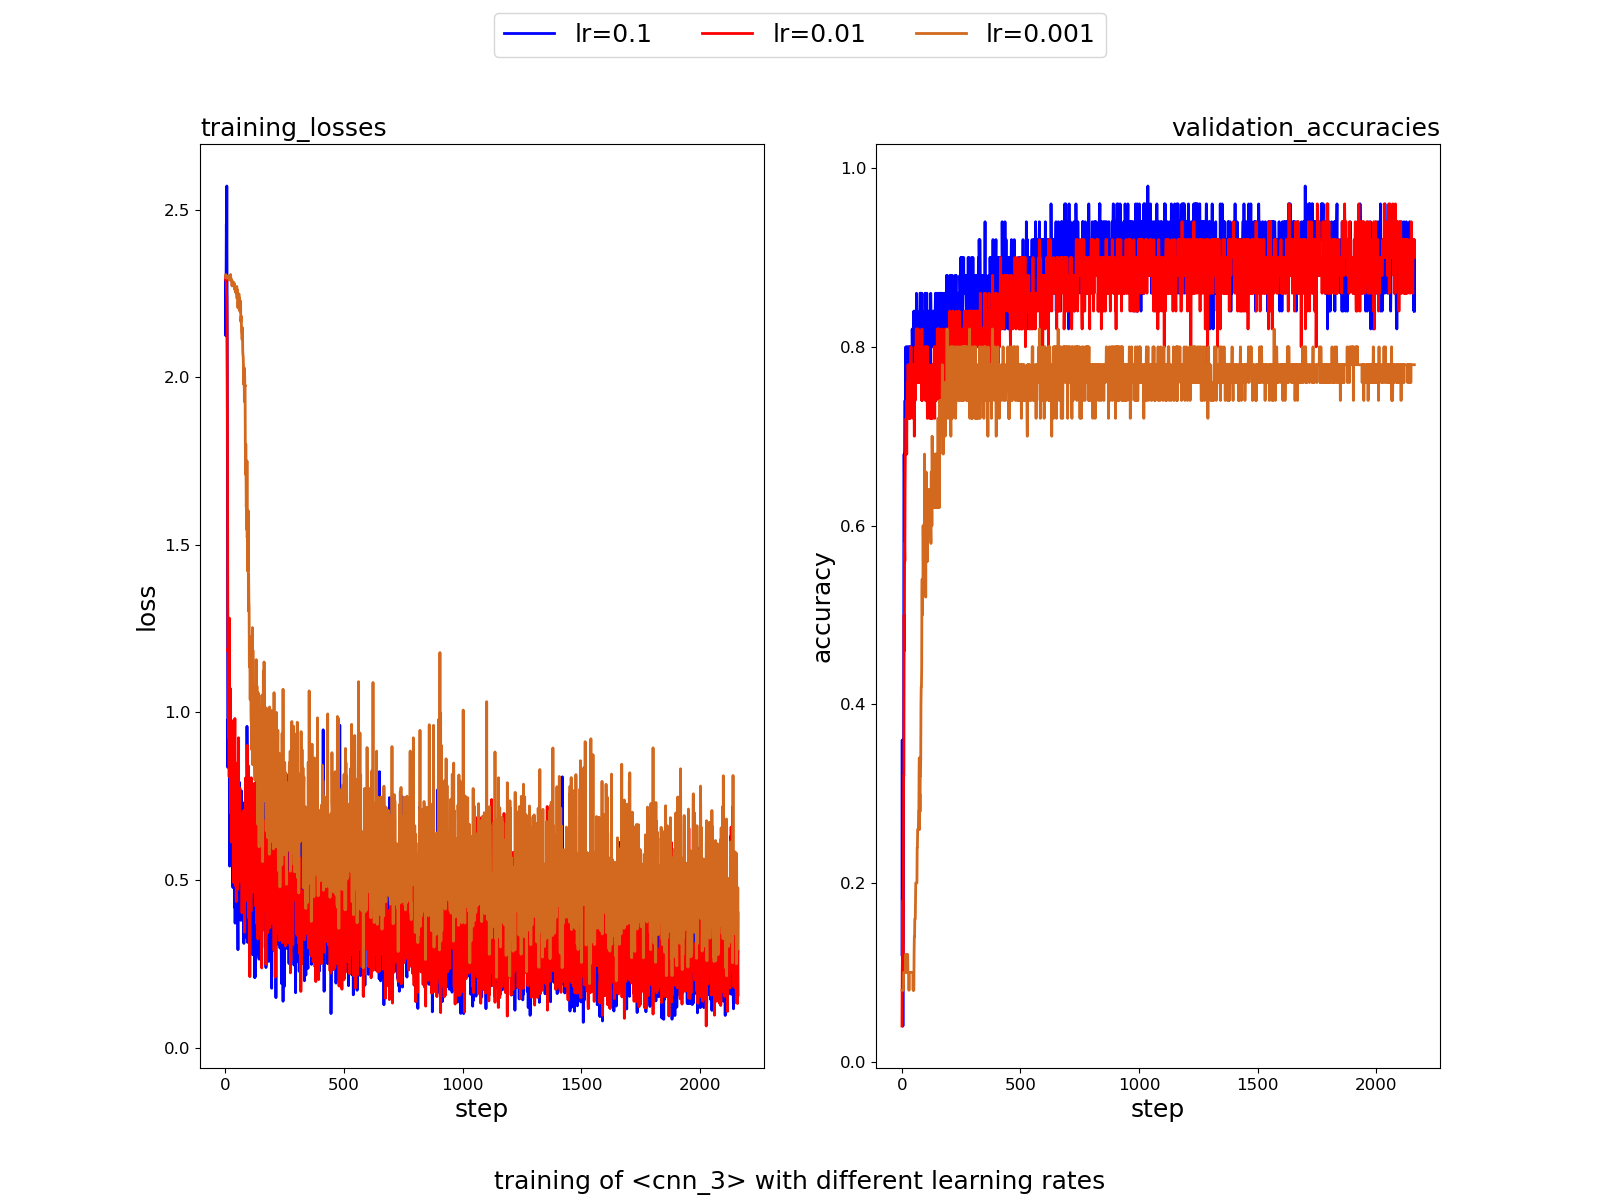
\includegraphics[width=1\textwidth]{figures/q5_1.png}
    \caption{Different learning rate settings on cnn3.}
    \label{fig:q5}
\end{figure}

\noindent Then scheduling is applied to the learning rate. Figure \ref{fig:q5_sch_1},\ref{fig:q5_sch_2},\ref{fig:q5_sch_3} illustrates the scheduling applied cases. The learning rate is decreased by a factor of 0.1 at each selected epoch.

\begin{figure}[!htb]
    \centering
    
\includegraphics[width=0.8\textwidth]{figures/part5_cnn_3_scheduled_1.png}
    \caption{No scheduling}
    \label{fig:q5_sch_1}
\end{figure}

\begin{figure}[!htb]
    \centering
    
\includegraphics[width=0.8\textwidth]{figures/part5_cnn_3_scheduled_2.png}
    \caption{LR dropped at 7th epch}
    \label{fig:q5_sch_2}
\end{figure}
\begin{figure}[!htb]
    \centering
    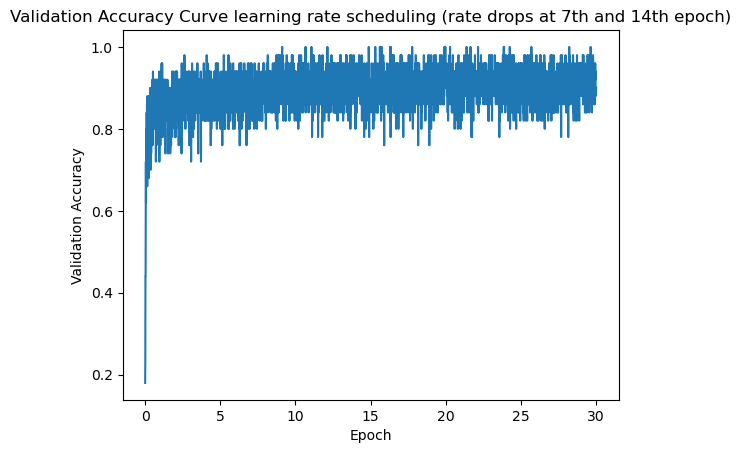
\includegraphics[width=0.8\textwidth]{figures/part5_cnn_3_scheduled_3.png}
    \caption{LR dropped at 7th and 15th epoch}
    \label{fig:q5_sch_3}
\end{figure}

\noindent It should be indicated that an inconsistent behavior for dropping the learning rate only for one case is observed. For example, when the exact same setup is run on different CUDA setups, the results are quite different, yet this also can be observed from the initial part of the b). This is repeated multiple times in different computation units. This was assumed to be an unsolved problem related to random initializations and seeds.

\subsection*{Question 5.2 - Discussions}

\textbf{1.}
\noindent As can be observed from Figure \ref{fig:q5}, as the learning rate increases, the convergence speed also increases.

\textbf{2.}
\noindent There are two points to consider when it comes to convergence to a better point. First, if the learning rate is too small, the weights may stuck at a suboptimal local minima. Also, even if the system convergence around the same minima, a small learning rate may lead to slow convergence. On the other hand, if the learning rate is too high, the weights may oscillate around the optimal point and may not go beyond a certain level. Therefore, the learning rate should be selected carefully. So, in order to find the best learning rate, one can start with a high learning rate and decrease it gradually. 

\textbf{3.}
\noindent In this case, the learning scheduling attempt worked out in terms of going to a better point. The oscillations around a convergence level are overcome by decreasing the learning rate. 

\textbf{4.}
\noindent When we compare these results with the one in question 3, where we trained the network with an ADAM optimizer, we can see that SGD yields a slightly better point. However, ADAM seems to converge faster than SGD. Yet, in this case, these two differences are quite subtle.
%--------------------------------------BIBLIOGRAFIA-------------------------------------------
\nocite{*} 


\end{document}